\section{Auswertung}
\label{sec:Auswertung}
Die Langmuir-Schottkysche Gleichung hat die Form $I = a \cdot U^b$. Diese lässt sich durch Logarithmisieren 
in die Geradengleichung 
    \begin{equation*}
    \log(I) = b \cdot \log(U) + \log(a)
    \end{equation*}
bringen. Zur Überprüfung der Gleichung wird eine lineare Regression der 5. Kennlinie verwendet, die bei dem 
höchsten Heizstrom entsteht. Durch die lineare Regression ergeben sich 
die Werte
\begin{align}
    \log(a) &= 1,26 \pm 0,02 \\
    b &= -6,28 \pm 0,08 \, .
\end{align}
$b$ ist zur Auswertung der Gültigkwit nicht relevant. $\log(a)$ kann mit dem Theoriewert $\log(a)_{\text{Theo}}= \frac{3}{2}$ verglichen werden.

% \begin{figure}
%   \centering
%   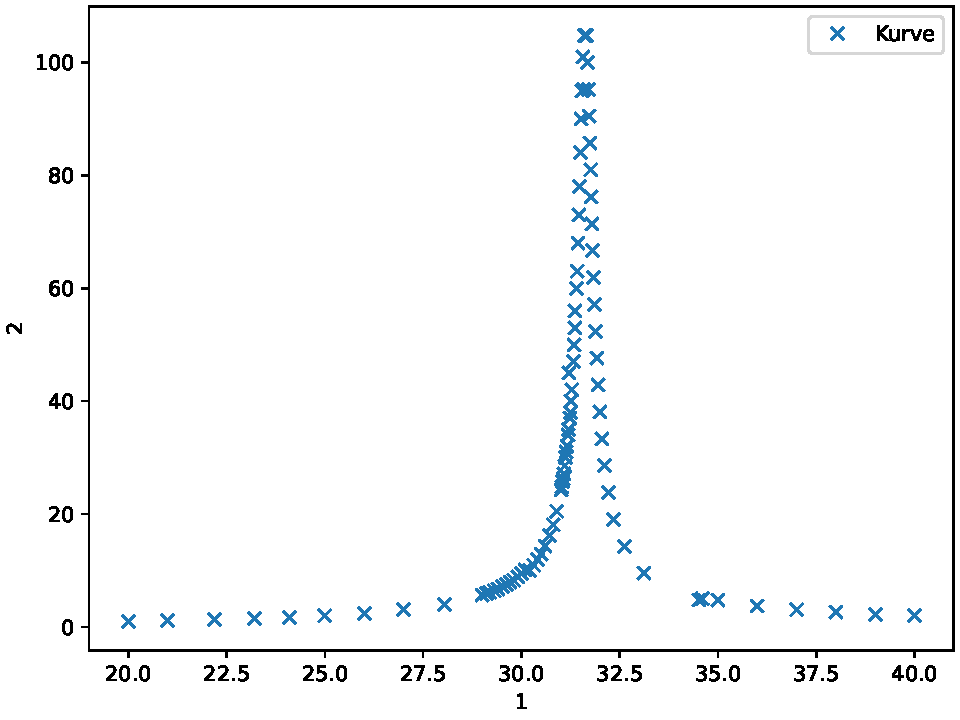
\includegraphics{plot.pdf}
%   \caption{Plot.}
%   \label{fig:plot}
% \end{figure}

%Siehe \autoref{fig:plot}!